\section{Exercises}

\begin{enumerate}[leftmargin=*]
\item Determine whether the statement is {\bf True} or {\bf False}.
\begin{enumerate}
\item Let $A$ be a $m$ by $n$ matrix such that $m > n$ and $\mathrm{rank}(A) = n$. There is a unique solution of $A \bs{x} = \bs{b}$ for any $\bs{b}$.
\item Let $A$ be a $m$ by $n$ matrix such that $m < n$ and $\mathrm{rank}(A) = m$. There are infinitely many solutions of $A \bs{x} = \bs{b}$ for any $\bs{b}$.
\item Let $A$ be a $m$ by $n$ matrix such that $m > n$ and $\mathrm{rank}(A) = n$. If the system $A \bs{x} = \bs{b}$ has one solution then there is only one solution.
\item Let $A$ be a $m$ by $n$ matrix such that $m > n$ and $\mathrm{rank}(A) < n$. If the system $A \bs{x} = \bs{b}$ has one solution then there are infinitely many solutions.
\item If $P$ is a permutation matrix such that $PA$ interchanges 2 rows of $A$, then $P^2 = I$.
\item If $A = PLU$ is the LU decomposition of $A$ with partial pivoting, then $| \ell_{i,j} | \leq 1$ for all $i > j$ where $\ell_{i,j}$ denotes the entry of $L$ at row $i$ and index $j$.
\item If $A = LU$ is the LU decomposition of $A$ without pivoting, then $| \ell_{i,j} | \leq 1$ for all $i > j$ where $\ell_{i,j}$ denotes the entry of $L$ at row $i$ and index $j$.
\item If $A = LU$ is the LU decomposition of $A$ then $\det(L) \not= 0$.
\item If $P$ is any permutation matrix and $L$ is unit lower triangular, then $P^{-1} L P$ is also unit lower triangular.
\item If $A$ is of the form
$$
A = \begin{bmatrix} * & * & 0 & 0 \\ * & * & * & 0 \\ 0 & * & * & * \\ 0 & 0 & * & * \end{bmatrix}
$$
and the $LU$ decomposition $A = LU$ exists, then $L$ and $U$ are of the form
$$
L = \begin{bmatrix} 1 & 0 & 0 & 0 \\ * & 1 & 0 & 0 \\ 0 & * & 1 & 0 \\ 0 & 0 & * & 1 \end{bmatrix}
\hspace{5mm}
U = \begin{bmatrix} * & * & 0 & 0 \\ 0 & * & * & 0 \\ 0 & 0 & * & * \\ 0 & 0 & 0 & * \end{bmatrix}
$$
\item If $\bs{x} \in \mathbb{R}^n$ such that $\| \bs{x} \|_1 = \| \bs{x} \|_{\infty} = \lambda$ then $\| \bs{x} \|_p = \lambda$ for any $p > 1$.
\item If $\| A \| = 1$ then $A = I$.
\item Define $\| \bs{x} \|_0 = \sum_{k=1}^n x_k^2$ for any $\bs{x} = \begin{bmatrix} x_1 & \cdots & x_n \end{bmatrix}^T \in \mathbb{R}^n$. Then $\| \bs{x} \|_{0}$ is a norm.
\item Define $\| \bs{x} \|_{\min} = \min_k | x_k |$ for any $\bs{x} = \begin{bmatrix} x_1 & \cdots & x_n \end{bmatrix}^T \in \mathbb{R}^n$. Then $\| \bs{x} \|_{\min}$ is a norm.
\item Consider $N+1$ data points $(t_0,y_0),\dots,(t_N,y_N)$. Let $A_1 \bs{c}_1 = \bs{b}_1$ be the linear system such that the solution $\bs{c}_1$ consists of the coefficients of the interpolating polynomial with respect to the monomial basis. Let $A_2 \bs{c}_2 = \bs{b}_2$ be the linear system such that the solution $\bs{c}_2$ consists of the coefficients of the interpolating natural cubic spline. Then we expect $\mathrm{cond}(A_1) < \mathrm{cond}(A_2)$ for large values of $N$.
\item Consider $d$ data points $(t_1,y_1),\dots,(t_d,y_d)$ (such that $t_i \not= t_j$). There exists a unique polynomial of degree (at most) $d-1$ which interpolates the data.
\item Consider $d$ data points $(t_1,y_1),\dots,(t_d,y_d)$ (such that $t_i \not= t_j$). There exists a unique polynomial $p(t)$ of degree (at most) $d$ which interpolates the data and also satisfies $p'(t_1)=0$ and $p''(t_1)=0$.
\item Consider $d$ data points $(t_1,y_1),\dots,(t_d,y_d)$ (such that $t_i \not= t_j$). There exists a unique polynomial $p(t)$ of degree (at most) $d$ which interpolates the data and $p'(t_1)=0$.
\item Consider $d+1$ data points $(t_0,y_0),(t_1,y_1),\dots,(t_d,y_d)$. Let $p(t)$ be the interpolating polynomial constructed using the monomial basis. Let $q(t)$ be the interpolating polynomial constructed using the Lagrange basis. Let $r(t)$ be the interpolating polynomial constructed using the Newton basis. Then $p(t) = q(t) = r(t)$ for all $t$.
\item The finite difference method applied to a linear second order differential equation with boundary conditions will compute exact values of the solution $y_k = y(t_k)$ if the step size $h$ is chosen to be small enough.
\item The finite difference method applied to a linear second order differential equation with boundary conditions  will never compute exact values of the solution $y_k = y(t_k)$ for any differential equation and step size $h$.
\end{enumerate}

\item Let $I$ be the identity matrix of size $n$ and let $R$ be the $n$ by $n$ matrix with all zeros except for the nonzero scalar $c$ at index $(i,j)$ where $i \not= j$. That is, the entry of $R$ in row $i$ and column $j$ is $c$ and all other entries of $R$ are 0. Let $E = I + R$ and let $A$ be any $n$ by $n$ matrix.
\begin{enumerate}
\item Matrix multiplication $EA$ is equivalent to which elementary row/column operation on $A$?
\item Matrix multiplication $AE$ is equivalent to which elementary row/column operation on $A$?
\end{enumerate}

%\item Compute the LU decomposition of
%$$
%A = \begin{bmatrix} 2 & 1 & 1 \\ 2 & 0 & 2 \\ 4 & 3 & 4 \end{bmatrix}
%$$

\item Find a value $c$ such that the system $A \bs{x} = \bs{b}$ has infinitely many solutions where
$$
A = \left[ \begin{array}{rrr} 3 & -1 & 2 \\ 1 & 1 & -1 \\ 2 & -2 & 3 \end{array} \right]
\hspace{5mm}
\bs{b} = \begin{bmatrix} 3 \\ 2 \\ c \end{bmatrix}
$$

\item Suppose Gaussian elimination without pivoting applied to a matrix $A$ produces the result
$$
L_3 L_2 L_1 A = U
$$
where
$$
L_1 = \begin{bmatrix} 1 & 0 & 0 & 0 \\ 1 & 1 & 0 & 0 \\ 3 & 0 & 1 & 0 \\ 2 & 0 & 0 & 1 \end{bmatrix}
\hspace{5mm}
L_2 = \begin{bmatrix} 1 & 0 & 0 & 0 \\ 0 & 1 & 0 & 0 \\ 0 & 2 & 1 & 0 \\ 0 & 5 & 0 & 1 \end{bmatrix}
\hspace{5mm}
L_3 = \begin{bmatrix} 1 & 0 & 0 & 0 \\ 0 & 1 & 0 & 0 \\ 0 & 0 & 1 & 0 \\ 0 & 0 & 4 & 1 \end{bmatrix}
$$
Determine the matrix $L$ in the decomposition $A = LU$.

\item Suppose we perform 2 iterations of Gaussian elimination with partial pivoting on a matrix $A$ such that the result is
$$
L_2 P_2 L_1 P_1 A = A_3 =
\begin{bmatrix} * & * & * & * \\ 0 & * & * & * \\ 0 & 0 & 2 & 1 \\ 0 & 0 & 5 & 4 \end{bmatrix}
$$
Determine the matrices $P_3$ and $L_3$ in the third step of the algorithm.

\item Let $P$ be the permutation matrix which moves row 3 to row 4, row 4 to row 5 and row 5 to row 3, and let 
$$
L = \begin{bmatrix} 1 & 0 & 0 & 0 & 0 \\ 0 & 1 & 0 & 0 & 0 \\ 0 & a & 1 & 0 & 0 \\ 0 & b & 0 & 1 & 0 \\ 0 & c & 0 & 0 & 1  \end{bmatrix}
$$
Determine $PLP^{-1}$.

\item Suppose $A$ is a symmetric positive definite matrix such that $A = LU$ where $L$ is unit lower triangular and 
$$
U = \begin{bmatrix} 4 & 1 & 0 & 3 \\ 0 & 1 & 2 & 1 \\ 0 & 0 & 9 & 5 \\ 0 & 0 & 0 & 1 \end{bmatrix}
$$
Find the Cholesky decomposition of $A$.

\item Suppose Gaussian elimination with partial pivoting applied to a matrix $A$ produces the result
$$
L_2 P_2 L_1 P_1 A = U
$$
where
$$
L_1 = \begin{bmatrix} 1 & 0 & 0 \\ 0.5 & 1 & 0 \\ 0.7 & 0 & 1 \end{bmatrix}
\hspace{5mm}
P_1 = \begin{bmatrix} 1 & 0 & 0 \\ 0 & 0 & 1 \\ 0 & 1 & 0 \end{bmatrix}
\hspace{5mm}
L_2 = \begin{bmatrix} 1 & 0 & 0 \\ 0 & 1 & 0 \\ 0 & 0.2 & 1 \end{bmatrix}
\hspace{5mm}
P_2 = \begin{bmatrix} 1 & 0 & 0 \\ 0 & 1 & 0 \\ 0 & 0 & 1 \end{bmatrix}
$$
Determine the matrices $P$ and $L$ in the decomposition $A = PLU$.

\item Suppose $A$ is a square matrix with LU decomposition $A = LU$ (where $L$ is unit lower triangular). Describe a method to compute $\det(A)$. Be specific.

\item Compute the Cholesky factorization of the matrix
$$
A = \begin{bmatrix} 2 & 1 & 0 \\ 1 & 2 & 1 \\ 0 & 1 & 2 \end{bmatrix}
$$

\item Find the solution of the system $A \bs{x} = \bs{b}$ for
$$
A = \left[ \begin{array}{rrr} 3 & 0 & \phantom{+}1 \\ -3 & -1 & 0 \\ 3 & -1 & 3 \end{array} \right]
\hspace{5mm}
\bs{b} = \left[ \begin{array}{r} 1 \\ -1 \\ 1 \end{array} \right]
$$
given the LU factorization
$$
A = LU
=
\left[ \begin{array}{rrr} 1 & \phantom{+}0 & \phantom{+}0 \\ -1 & 1 & 0 \\ 1 & 1 & 1 \end{array} \right]
\left[ \begin{array}{rrr} 3 & 0 & \phantom{+}1 \\ 0 & -1 & 1 \\ 0 & 0 & 1 \end{array} \right]
$$

\item Suppose we compute a decomposition $A = L_0U_0$ such that $U_0$ is {\it unit} upper triangular and $L_0$ is lower triangular. Describe a method to derive a decomposition $A = LU$ such that $L$ is {\it unit} lower triangular and $U$ is upper triangular.

\item Suppose $A$ is a 2 by 2 matrix such that the image of the unit circle under the linear transformation given by $A$ is:
\begin{center}
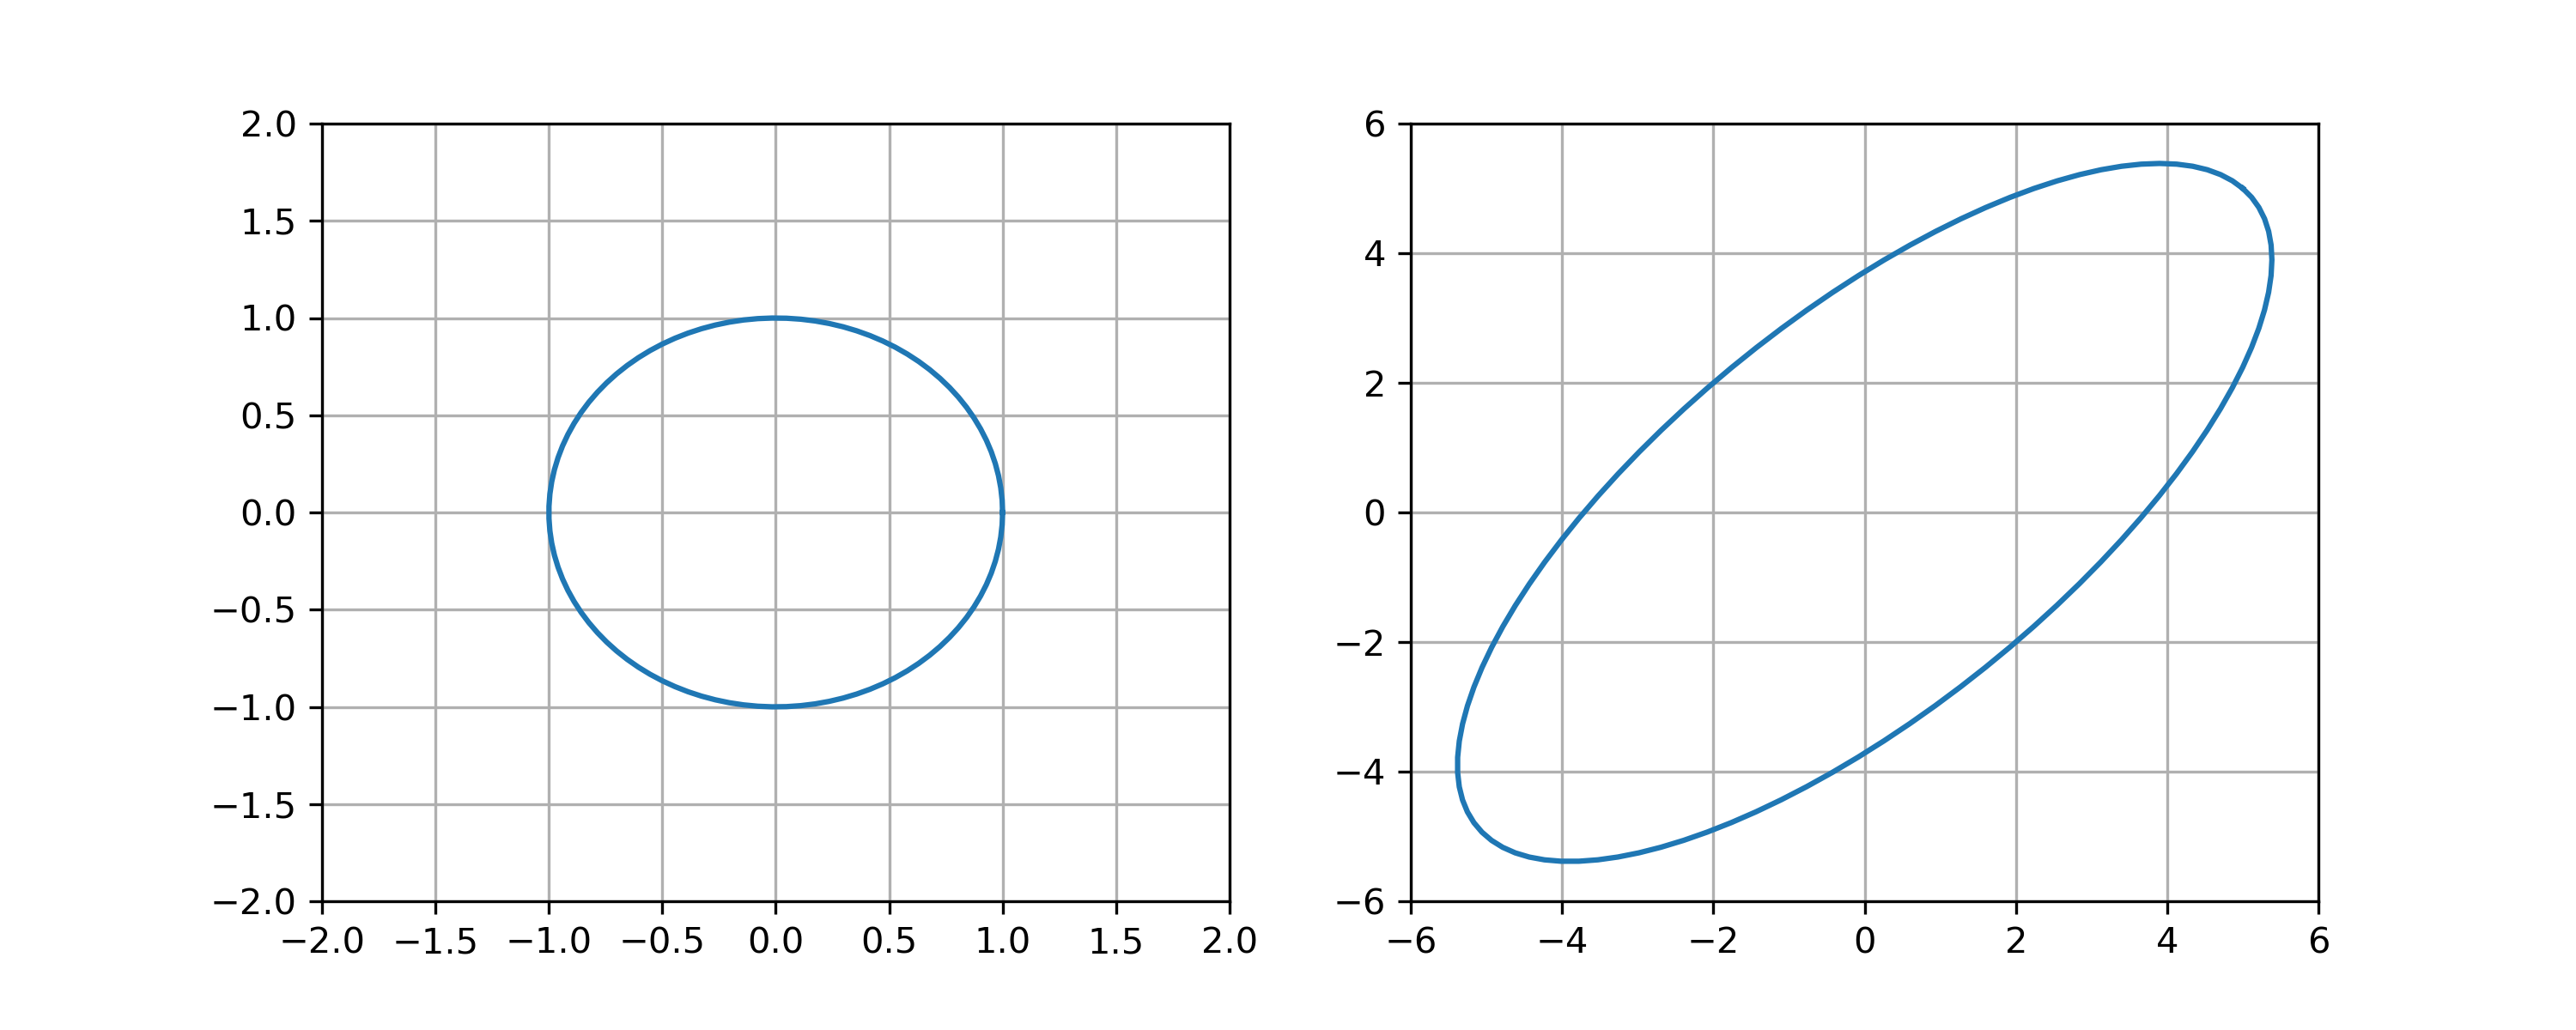
\includegraphics[width=6in]{img01b.png}
\end{center}
Determine $\mathrm{cond}_2(A)$ (the condition number with respect to the 2-norm).

\item Suppose $\bs{x} = \begin{bmatrix} 1 & 2 & 2 & c & 1 & 1 \end{bmatrix}^T \in \mathbb{R}^6$ such that $\| \bs{x} \|_{3} = 3$. Find all possible values $c$.

\item Suppose $\bs{x} = \begin{bmatrix} 1 & 3 & 2 & 2 & c & 2 & 1 & 2 \end{bmatrix}^T \in \mathbb{R}^8$ such that $\| \bs{x} \|_{3} = 5$. Find all possible values $c$.

\item Suppose $\bs{x} = \begin{bmatrix} 1 & 0 & 2 & c & -1 \end{bmatrix}^T \in \mathbb{R}^5$ such that $\| \bs{v} \|_1 = 5$. Find all possible values $c$.

\item Suppose $\bs{x} = \begin{bmatrix} 1 & 0 & 2 & c & -1 \end{bmatrix}^T \in \mathbb{R}^5$ such that $\| \bs{x} \|_{\infty} = 5$. Find all possible values $c$.

\item Suppose $A$ is a 2 by 2 matrix such that the image of the unit square under the linear transformation given by $A$ is:
\begin{center}
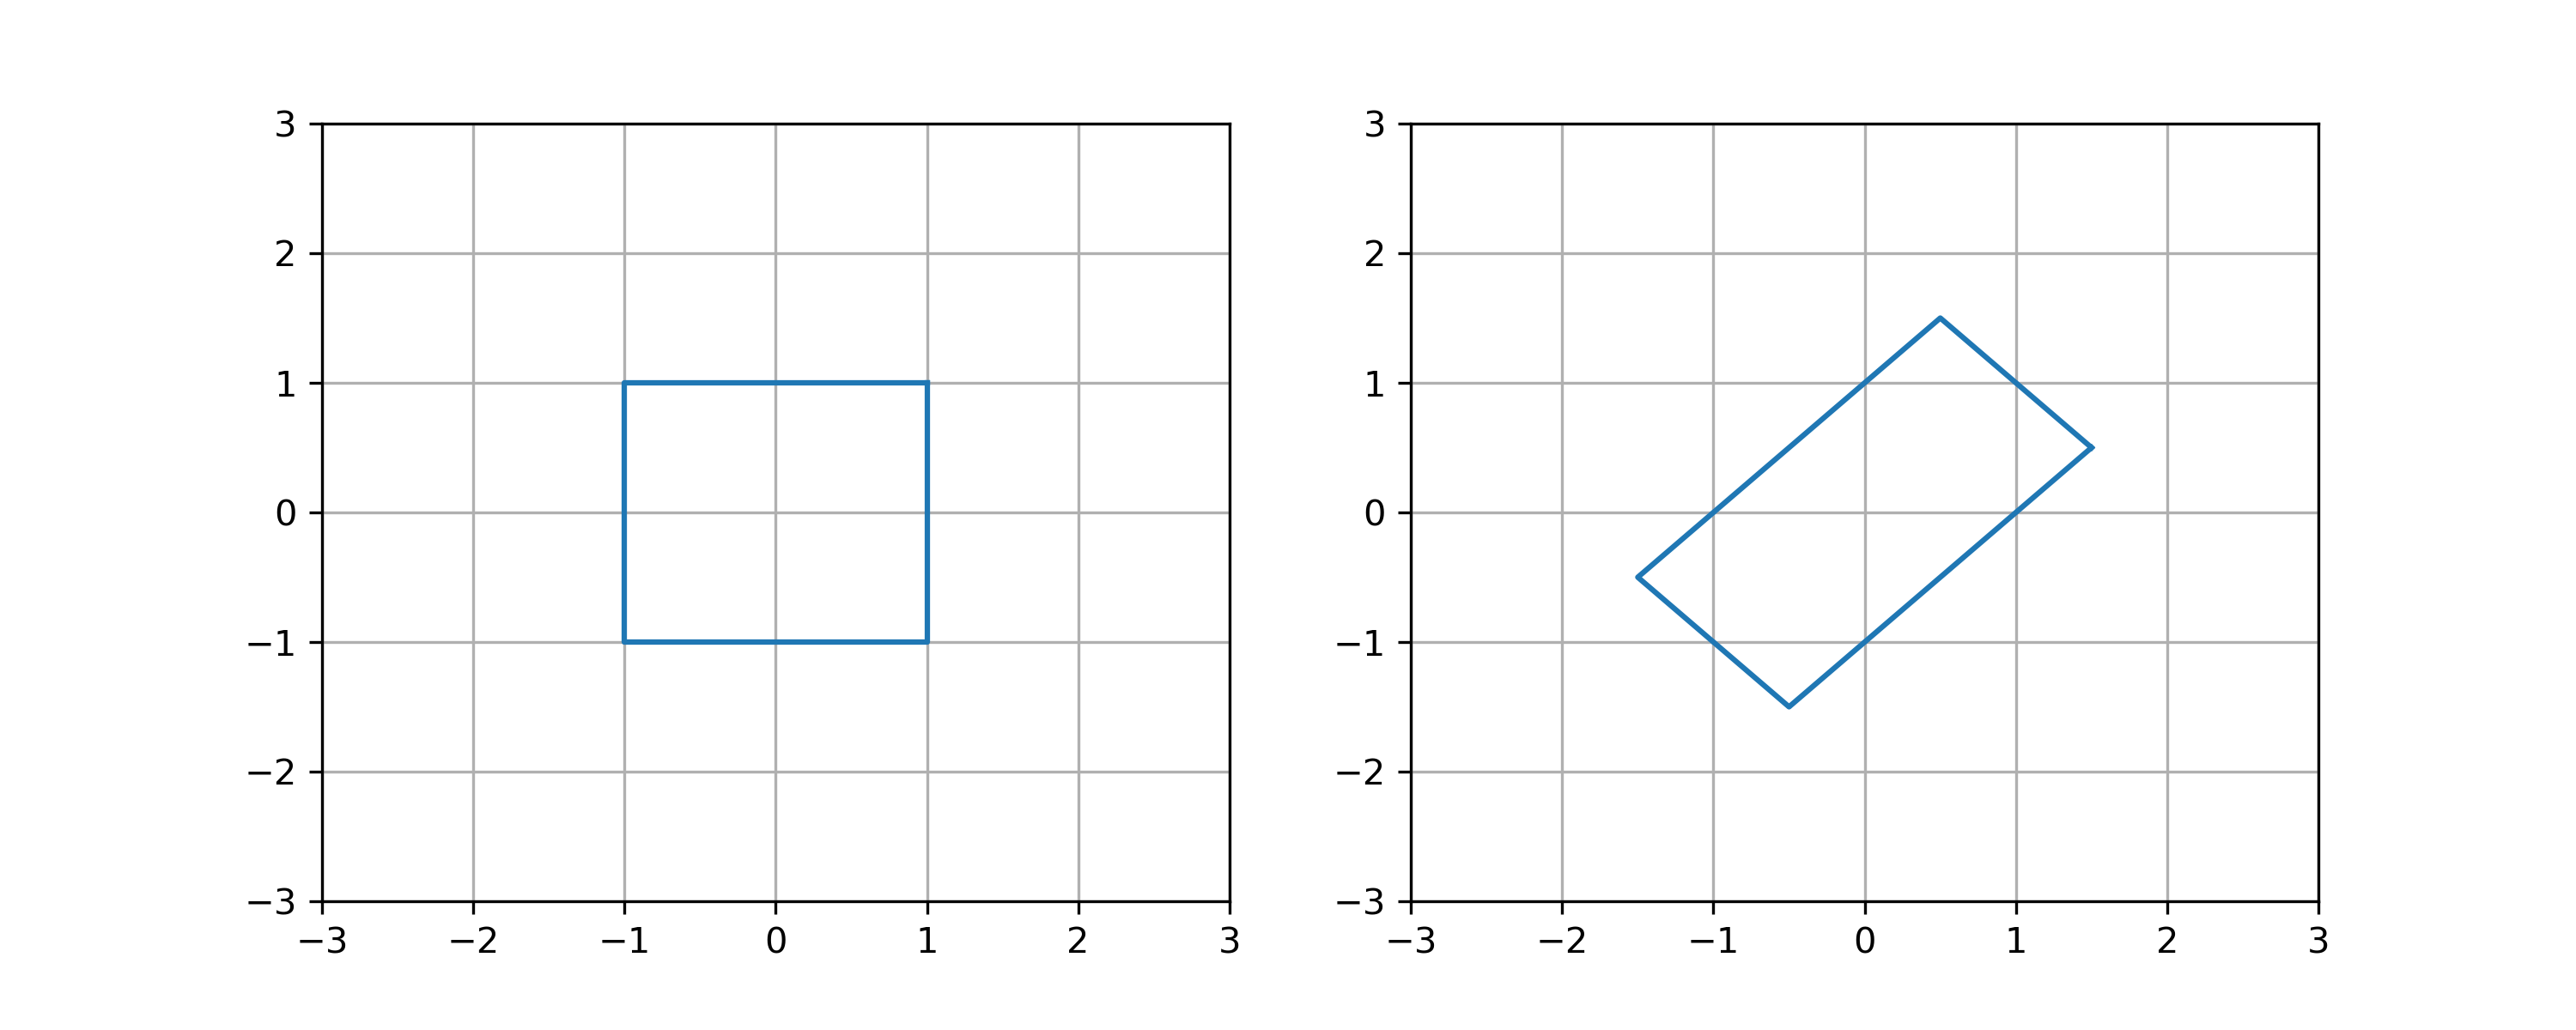
\includegraphics[width=6in]{img02.png}
\end{center}
Determine $\mathrm{cond}_{\infty}(A)$ (the condition number with respect to the $\infty$-norm).

\item Suppose $A$ is a 2 by 2 matrix such that the image of the unit ``diamond" under the linear transformation given by $A$ is:
\begin{center}
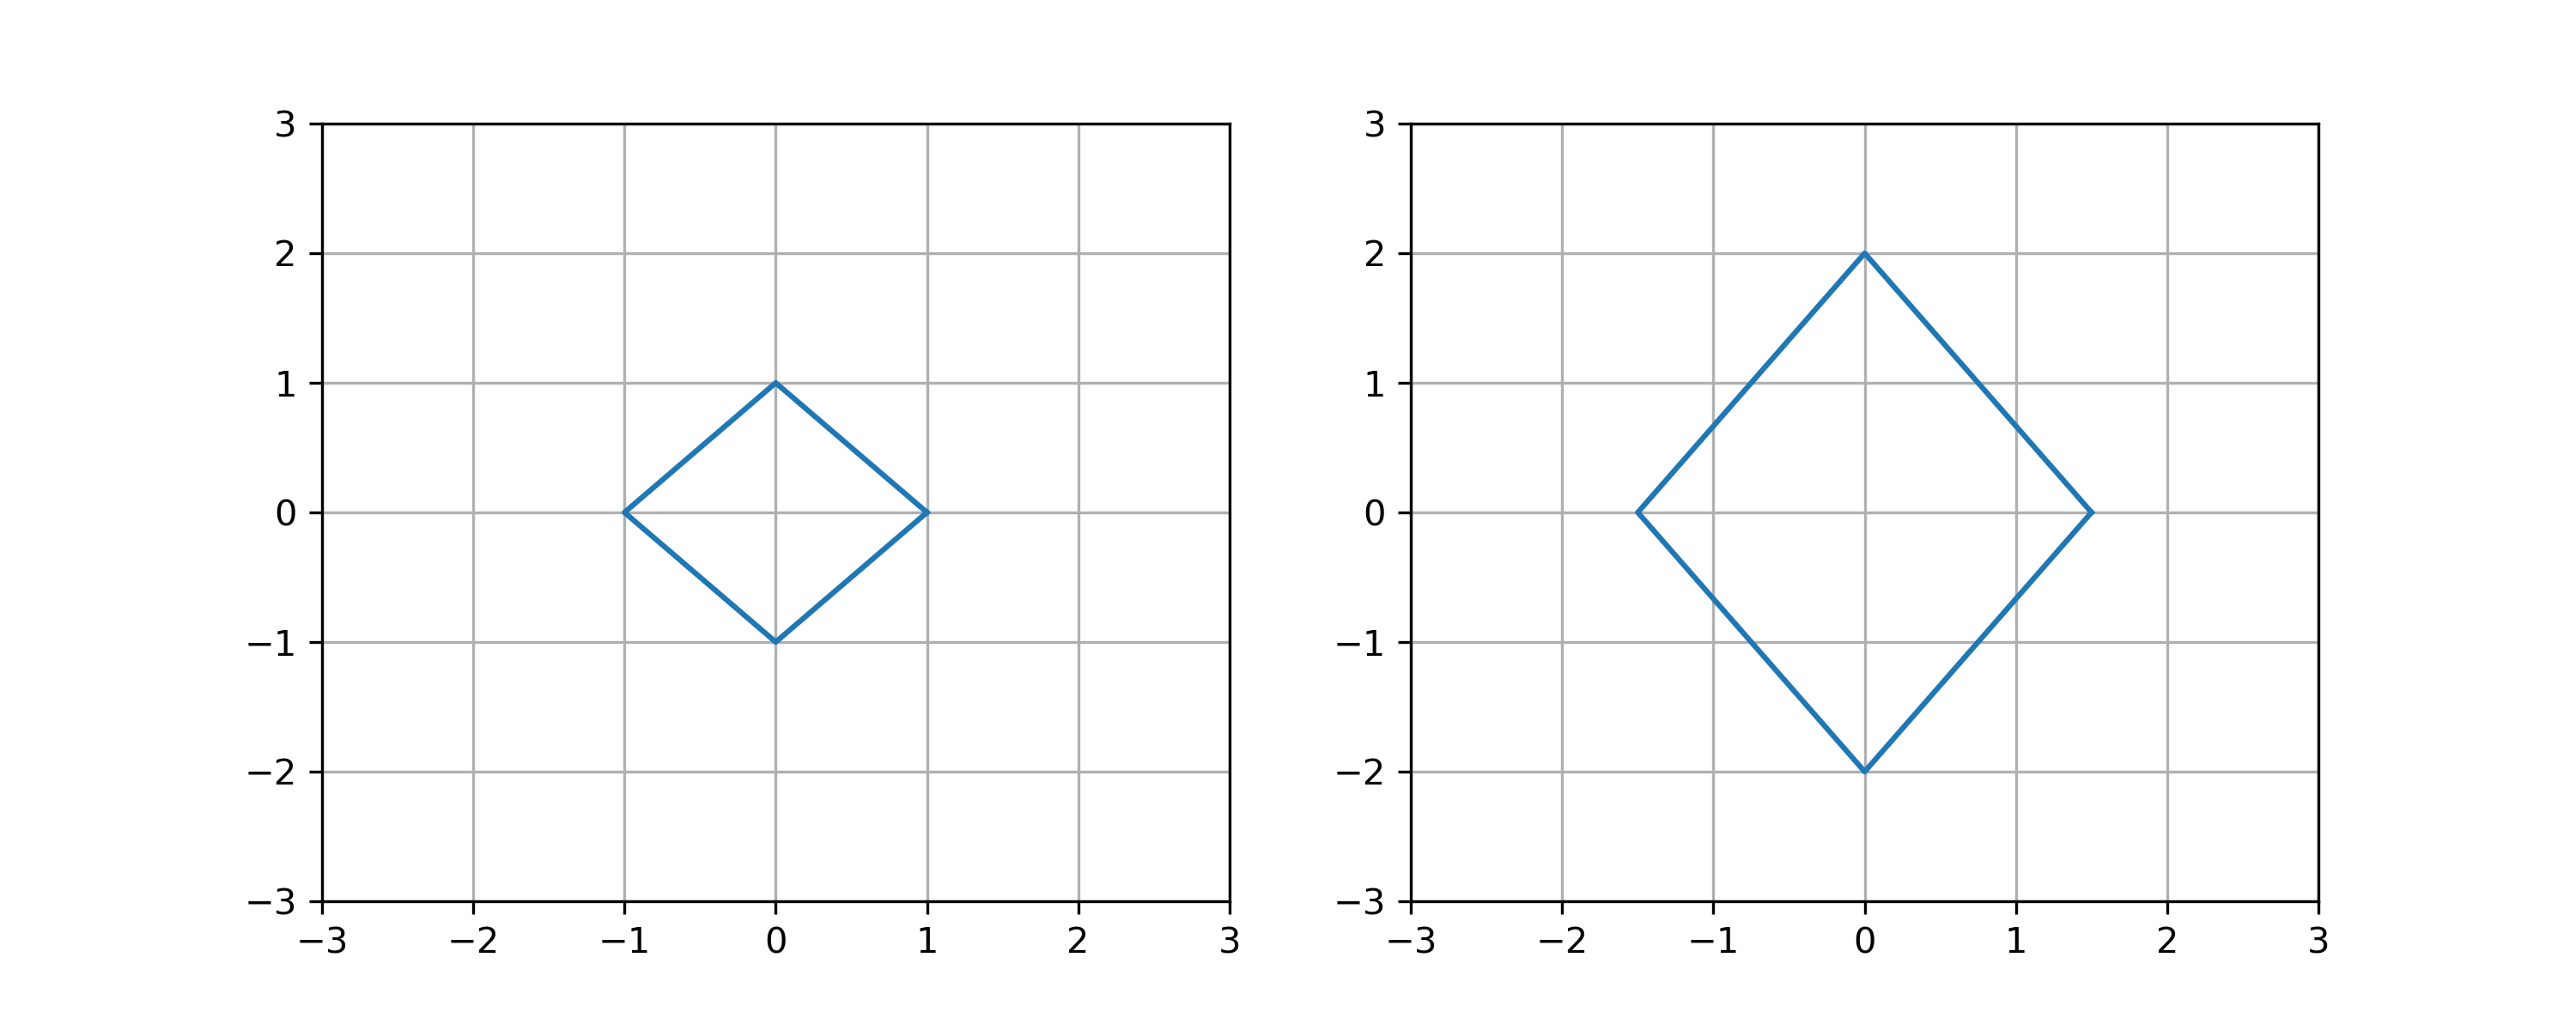
\includegraphics[width=6in]{img03.png}
\end{center}
Determine $\mathrm{cond}_1(A)$ (the condition number with respect to the 1-norm).

\item Suppose we have 4 points $(0,y_0),(1,y_1),(2,y_2),(3,y_3)$ and we want to interpolate the data using a spline $p(t)$ constructed from $3$ degree 2 polynomials $p_1,p_2,p_3$ where
$$
p_k(t) = a_k(t - t_{k-1})^2 + b_k(t - t_{k-1}) + c_k \ \ , \ \ t \in [t_{k-1},t_k]
$$
We require that $p(t)$ and $p'(t)$ are continuous and $p''(t_0)=0$. Setup a linear system $A \bs{x} = \bs{b}$ where the solution is
$$
\bs{x} = \begin{bmatrix} a_1 & b_1 & a_2 & b_2 & a_3 & b_3 \end{bmatrix}^T
$$
Note: the system depends on the unspecified values $y_0,y_1,y_2,y_3$.

\item Suppose a cubic spline $p(t)$ interpolates the data
$$
(0.0,0.0),(1.0,2.0),(2.0,1.0),(3.0,3.0),(4.0,-1.0),(5.0,1.0)
$$
and $p(t)$ has coefficient matrix
$$
\left[ \begin{array}{rrrrr}
1.9 & 1.9 & a_3 & 3.1 & 3.1 \\
-7.2 & -1.5 & b_3 & -6.3 & 3.0 \\
7.3 & -1.4 & c_3 & -0.8 & -4.1 \\
0.0 & 2.0 & 1.0 & 3.0 & -1.0
\end{array}\right]
$$
Determine the coefficients $a_3,b_3,c_3$.

\item Suppose a cubic spline $p(t)$ interpolates the data
$$
(0.0,1.0),(1.0,3.0),(2.0,1.0),(3.0,1.0),(4.0,2.0),(5.0,1.0)
$$
and $p(t)$ has coefficient matrix (rounded to 2 decimal places)
$$
\left[\begin{array}{rrrrr}
-1.19 & 1.93 & a_3 & -0.75 & 0.55 \\
0.00 & -3.56 & b_3 & 0.60 & -1.65 \\
3.19 & -0.37 & c_3 & 1.15 & 0.10\\
1.00 & 3.00 & 1.00 & 1.00 & 2.00
\end{array} \right]
$$
Determine the coefficients $a_3,b_3,c_3$.

\item Suppose we discretize the domain $[0,1]$ of a differential equation with boundary conditions
$$
y'' + p(t)y' + q(t)y = r(t) \ \ , \ \ y(0) = \alpha \ \ , \ \ y(1) = \beta
$$ 
with step size $h=0.1$ and derive a linear system $A \bs{y} = \bs{b}$. How many unknown values $y_k$ are we solving for in this case?

\item Setup a linear system $A \bs{y} = \bs{b}$ to approximate the solution of the equation with boundary conditions
$$
y'' = 2^t \ \ , \ \ y'(0) = 1 \ , \ \ y(1) = 0
$$
using step size $h=0.25$. Use the forward difference formula and the boundary condition $y'(0)=0$ to approximate the boundary value $y_0$.

\item Derive the general form of the linear system $A \bs{y} = \bs{b}$ for an equation with boundary conditions
$$
y'' + p(t)y' = r(t) \ \ , \ \ y(t_0) = \alpha \ \ , \ \ y(t_f) = \beta
$$
using the forward difference formula to approximate $y'$. Use the notation as in the examples: choose $N$, let  $h = (t_f - t_0)/(N+1)$ and $t_k = t_0 + kh$, let $y_k$ denote an approximation of $y(t_k)$ and note $y_0 = \alpha$ and $y_{N+1} = \beta$.

\item Explain why it is not possible to derive a linear system $A \bs{y} = \bs{b}$ for the equation
$$
y' = \cos(y) \ \ , \ \ y(0) = 0 \ \ , \ \ y(1) = \frac{\pi}{4}
$$
by applying finite difference formulas.

\item Suppose we compute the finite difference approximation of the equation
$$
y'' = \frac{5}{1 + t^4} \ \ , \ \ y(0) = 0 \ \ , \ \ y(1) = 1
$$
with 5 equally spaced points from $t_0 = 0$ to $t_4 = 1$ and find $y_1 = -0.19554177$ and $y_3 = 0.35872678$. Determine $y_2$.
%y = [-0.19554177, -0.06757813,  0.35872678]

\item Setup a linear system $A \bs{y} = \bs{b}$ for the finite difference approximation of
$$
y'' + ty = 0 \ \ , \ \ y(1) = 1 \ \ , \ \ y(3) = -1
$$
using 5 equally spaced points from $t_0 = 1$ to $t_4 = 3$.

\item Setup a linear system $A \bs{y} = \bs{b}$ for the finite difference approximation of
$$
y'' + ty = 0 \ \ , \ \ y(1) = 1 \ \ , \ \ y'(3) = -1
$$
using 5 equally spaced points from $t_0 = 1$ to $t_4 = 3$. (Hint: use the backwards difference formula to approximate $y_4$.)

\item Setup the linear system $A \boldsymbol{y} = \boldsymbol{b}$ corresponding to the finite difference method applied to the equation
$$
y'' + y' = t^2 \ \ , \ \ y(-1) = y(1) = 0
$$
using 9 equally spaced points on the domain $[-1,1]$.

\item Setup the linear system $A\bs{y} = \bs{b}$ corresponding to the finite difference method applied to the equation
$$
y'' + \cos(t) y = \sin(t) \ \ , \ \ y(0) = y(2\pi) = 0
$$
using 9 equally spaced points on the domain $[0,2\pi]$.

\item Setup the linear system $A\bs{y} = \bs{b}$ corresponding to the finite difference method applied to the equation
$$
y'' + \sin(t) y = \cos^2(t) \ \ , \ \ y(0) = y(2\pi) = 0
$$
using 9 equally spaced points on the domain $[0,2\pi]$.

\end{enumerate}